% MA-SQLGrid original-title reconstruction, Applied Sciences R3.
\documentclass[applsci,article,submit,moreauthors]{Definitions/mdpi}
\firstpage{1}
\makeatletter\setcounter{page}{\@firstpage}\makeatother
\pubvolume{1}\issuenum{1}\articlenumber{0}\pubyear{2026}\copyrightyear{2026}
\datereceived{}\daterevised{}\dateaccepted{}\datepublished{}
\usepackage{booktabs}
\usepackage{algorithm}
\usepackage{algorithmic}
\setlength{\headheight}{20pt}
\setlength{\emergencystretch}{3em}
\newcommand{\masql}{MA-SQLGrid}
\AtBeginDocument{\pdfstringdefDisableCommands{\def\times{x}}}

\Title{MA-SQLGrid: A Robust Multi-Agent Framework for Text-to-SQL in Power Grid Databases}
\Author{Liu Bijing $^{1,2}$, Sun Chenglong $^{1,2}$ and Yang Yong $^{1,2,}$*}
\AuthorNames{Liu Bijing, Sun Chenglong and Yang Yong}
\address{$^{1}$ \quad NARI Group Corporation (State Grid Electric Power Research Institute), Nanjing 211106, Jiangsu Province, China;\\
$^{2}$ \quad Beijing Kedong Electric Power Control System Co., Ltd., Beijing 100080, China}
\corres{Correspondence: Yang Yong; email address to be provided before submission}

\abstract{Natural-language access to power-grid databases requires traceable schema grounding, database-enforced read-only execution, and explicit treatment of missing evidence. This paper presents \masql{}, a five-role software architecture coordinated through an append-only blackboard and deterministic adjudicator. The implemented boundary uses SQLite read-only mode, \texttt{query\_only}, an authorizer, disabled extensions, resource limits, and fail-closed named-state coverage. Earlier GridDB and BIRD experiments evaluate frozen prompting workflows, not autonomous multi-agent generation. The only audited prospective experiment is a separate 700-call component study; it tests presented-value and reference-free selection components rather than the five-role system. A deterministic no-generation release-v3 re-execution applies three selectors to a shared 5760-attempt evidence collection for eight historical candidates on 180 GridDB questions. A supersession record classifies this release as descriptive because its frozen pre-run tests accessed same-item gold-derived v2 outcomes. Fixed order, validation-only ranking, and complete three-witness selection obtained 80/180, 100/180, and 101/180, respectively. The latter two selectors had top-score ties on 130/180 questions, with mean tie multiplicities 5.4000 and 5.3889; reversing candidate order yielded 117--118/180. Their sole difference was Q039, where a constructed nullable-column witness rejected \texttt{SELECT *} and retained an explicit projection. This 1/180 trace is semantically ambiguous and is not evidence of a general counterfactual, robustness, coordination, or multi-agent gain. The evidence supports a reproducible architecture with tested safety and bounded-evidence mechanisms, but not end-to-end agent superiority, qualified power-grid semantic validity, deployment safety, or universal robustness.}
\keyword{text-to-SQL; multi-agent systems; power-grid databases; schema grounding; execution validation; counterfactual testing; reproducibility}
\featuredapplication{\masql{} is an experimental read-only decision-support framework for auditable natural-language access to structured power-grid records. Generated SQL and returned source rows require human inspection before consequential use; no operational control, protection, or maintenance decision has been validated.}

\begin{document}

\section{Introduction}

Power-grid organizations maintain relational data about assets, locations, topology, sensor readings, work orders, technicians, and maintenance activity. SQL provides precise access to these records, but it requires knowledge of table names, join keys, identifiers, units, aggregation conventions, and local coding rules. Text-to-SQL systems aim to reduce this access barrier by translating a natural-language request into an executable query. In an engineering workflow, however, a fluent query is not sufficient evidence of correctness. A query can execute while selecting the wrong status field, omitting a required filter, using an unintended join path, or returning the expected number of columns with the wrong content.

Cross-database benchmarks such as Spider and BIRD have made schema generalization and realistic database content central evaluation concerns \cite{yu2018spider,li2023bird}. Schema-aware models, constrained decoding, context selection, decomposition, and execution guidance address different failure surfaces \cite{wang2020ratsql,scholak2021picard,nan2023enhancing,pourreza2023dinsql,talaei2024chess}. These methods also expose a design problem: generation steps are frequently bundled together. A system may change schema serialization, value presentation, domain normalization, structural hints, candidate count, and repair policy simultaneously. An observed score difference then cannot be assigned cleanly to schema linking, reasoning, or validation.

The original \masql{} concept addresses this problem through five specialized roles. A Query Analyst interprets the request, a Schema Cartographer maps it to the database, an SQL Synthesizer packages candidate queries, a Validation Engine checks safety and execution, and a Counterfactual Critic records evidence from named database states. A separate deterministic adjudicator resolves the resulting evidence. This separation makes the trace inspectable: a reviewer can distinguish what the analyst inferred, which schema elements were retained, which candidates were proposed, which candidates executed, and why a final candidate was selected or rejected.

The architecture must nevertheless be separated from the evidence used to evaluate it. The inherited GridDB factorial study was not a multi-agent execution. It used one model generation per question and prompt cell, followed by deterministic parsing, read-only validation, execution, and offline scoring. The BIRD study likewise compared four frozen prompting procedures rather than five interacting agents. These assets can motivate modules, supply baselines, and test replay interfaces, but they cannot be renamed as results of the new coordination core.

This distinction leads to three questions. First, can role-specific handoffs be implemented with a database-enforced, gold-isolated, fail-closed boundary? Second, what do the completed experiments establish about context packages, presented values, public-database transfer, and constructed-state agreement? Third, when generation is held fixed at eight already frozen candidates per question, how do fixed-order, validation-only, and complete metamorphic selectors behave under the same evidence-collection operations? The third question estimates historical-pool offline selection only; schema grounding is retained as trace evidence and no five-role end-to-end, new-generation, dialogue, or deployment effect is estimated.

The paper makes four contributions. First, it defines a testable five-role coordination core, a database-enforced SQLite executor, and a deterministic adjudicator whose required counterfactual coverage fails closed. Second, it conservatively integrates a 1440-prediction GridDB factorial experiment, an audited prospective 700-call component study, a 25,920-row multi-state ledger, and a 5000-call BIRD comparison while retaining their original identities and evidence classes. Third, it reports a deterministic descriptive re-execution over the existing eight-slot pool using three query-blind metamorphic witnesses with distinct database hashes; all methods choose only after the same shared 32-attempt evidence collection per question is complete. Fourth, it publishes complete counts and adverse diagnostics: 130/180 top-score ties for both adjudicating selectors, approximately 5.4 candidates per top-tie set, all 18 order/weight/threshold cells, and the semantically ambiguous 1/180 Q039 trace.

No Spider or WikiSQL experiment is reported, no unsupported large power-grid question--SQL corpus is asserted, and the offline result is not relabeled as autonomous multi-agent generation. In the retained title, \emph{multi-agent} names the typed five-role software decomposition, not five concurrently hosted language models, and \emph{robust} names only the explicitly tested mutation-denial, bounded-execution, complete-evidence, and three-witness mechanisms. The title is therefore a framework identity rather than an empirical superiority claim. Qualified domain review and a matched new-generation experiment remain mandatory gates before broader interpretation.

\section{Related Work}

\subsection{Text-to-SQL Evaluation and Schema Generalization}

Text-to-SQL systems map a natural-language question and a database schema to a query. Spider established a cross-domain setting with previously unseen databases, drawing attention to table selection, joins, grouping, nesting, and ordering \cite{yu2018spider}. BIRD extends public evaluation toward larger and more content-rich databases \cite{li2023bird}. A benchmark result depends on the exact split, evaluator, database engine, execution boundary, and model configuration. We therefore report only the completed BIRD Mini-Dev protocol and make no claim about public datasets that were discussed but not run.

Exact SQL match and execution evaluation answer different questions. String match can penalize equivalent SQL, whereas result equality can reward nonequivalent queries on an insufficiently discriminating database state. A robustness evaluation should retain predicted SQL, record every failure, and specify the state on which equality was observed. \masql{} uses strict result equality for inherited snapshot analyses and separately reports constructed-state agreement and bounded metamorphic invariance. Neither auxiliary endpoint is semantic certification.

\subsection{Schema Linking, Context Packages, and Output Contracts}

Schema linking connects question spans to tables, columns, values, and foreign-key relations \cite{wang2020ratsql,lei2020reexamining,liu2022semantic}. Full-schema context preserves recall but can increase token cost and distraction. Compact context reduces the search space but risks dropping a required join key or predicate. Value examples can disambiguate coded attributes, while question-derived instructions can identify aggregation, result shape, ordering, or a limit.

The inherited GridDB factorial study isolates two implemented prompt factors: a full-DDL/global-values package versus a compact/domain-grounded package, and absence versus presence of a composite structural/SQL-operation hint. The compact package is not a pure schema-length manipulation because it also changes value presentation and adds corpus-tailored normalization. The hint is not merely formatting because it can include aggregation, grouping, projection, ordering, and limit guidance. We retain these precise labels instead of assigning broader causal interpretations.

Constrained generation and execution guidance reduce invalid candidates. PICARD constrains decoding so inadmissible SQL continuations can be rejected during generation \cite{scholak2021picard}. CHESS combines contextual grounding and SQL synthesis components \cite{talaei2024chess}; other prompt-based methods investigate decomposition and representation choices \cite{nan2023enhancing,sun2023sqlprompt,pourreza2023dinsql}. \masql{} differs at the coordination boundary: its new core accepts externally produced candidates, checks them with deterministic contracts, and records evidence before selection. It does not claim that the current lexical cartographer supersedes learned schema-linking systems.

\subsection{Agentic Decomposition and Auditable Control}

Agentic decomposition can make intermediate decisions explicit, but naming pipeline stages as agents does not establish a multi-agent benefit. Such evidence requires a comparison that holds the model, data, decoding configuration, candidate count, and physical generation budget constant. Otherwise, a multi-candidate system can improve simply because it receives more samples.

\masql{} treats an agent as a role with a typed contract rather than assuming that every role must be a separately hosted model. The Analyst and Cartographer can be deterministic or model-assisted; the Synthesizer can receive candidates from a frozen generator; the Validator uses a fixed read-only policy; the Critic consumes named-state evidence; and the Adjudicator is deterministic. This design allows components to be replaced without changing the blackboard schema and prevents gold-guided selection from being hidden behind an opaque debate label.

\subsection{Power-Grid Data and External Validity}

Power-system datasets combine topology, equipment attributes, measurements, time series, costs, and constraints. RTS-GMLC and SimBench provide reproducible engineering resources that can be transformed into relational structures \cite{barrows2020rts,meinecke2020simbench}. Their availability does not automatically create a text-to-SQL benchmark: intended projections, units, ordering, ties, and reference SQL require semantic review. The current RTS-GMLC, SimBench, and NERC-derived candidates are consequently machine-adjudicated silver resources, not expert gold.

DKA-SQL is a direct power-grid text-to-SQL precedent \cite{bian2025dkasql}. Its published corpus, method, models, and evaluation boundary differ from ours. Because no official implementation was used, the current BIRD protocol is neither a DKA-SQL reproduction nor a head-to-head comparison.

\section{Materials and Methods}

\subsection{Task and Evidence Boundary}

For question $x_i$, read-only database $D_i$, and introspected schema $S_i$, a generator produces one or more candidates
\begin{equation}
\mathcal{Y}_i=\{\widetilde{y}_{i1},\ldots,\widetilde{y}_{ik}\}.
\end{equation}
Each candidate must satisfy a single-statement read-only contract. The accepted leading form is \texttt{SELECT} or \texttt{WITH}; comments, multiple statements, write operations, schema changes, attachments, and pragmas are rejected. A candidate is eligible for adjudication only when it is safe and executable.

The offline evaluator may later compare the selected query with a reference result. Let $E_i=1$ when the selected SQL executes and its result equals the frozen reference result under the registered evaluator, and $E_i=0$ otherwise. Reference SQL, reference results, $E_i$, and any derivative correctness field are forbidden from all five agents and the Adjudicator. Evaluation occurs only after the blackboard is sealed.

\subsection{Data Resources and Provenance}

GridDB-Maintenance-v2 v0.1 is a synthetic SQLite case study with eight tables and 98 rows: \texttt{asset\_types} (6), \texttt{assets} (18), \texttt{grid\_topology} (9), \texttt{locations} (8), \texttt{maintenance\_logs} (8), \texttt{sensor\_readings} (26), \texttt{technicians} (8), and \texttt{work\_orders} (15). It contains 200 natural-language--SQL records: 20 development records and 180 factorial evaluation records. The evaluation records include 66 easy, 91 medium, and 23 hard items and map to 70 normalized gold-SQL structural clusters, of which 58 are singletons. The evaluation partition had been visible during project development; it is a controlled finite-set case study, not a sealed production benchmark.

BIRD Mini-Dev contributes 500 public items over 11 SQLite databases. The authorized protocol froze item and method order, prompts, two local model files, evaluator behavior, Python 3.10.11/SQLite 3.40.1, and zero retries. Each backbone made 2500 calls and produced 2000 final predictions. An independent audit re-executed all 4000 predictions and 500 gold queries with zero score mismatches. Two earlier failed attempts, totaling 2476 physical calls, remain immutable incidents and are excluded from scores.

The GridDB reliability release contains 18 states: the canonical snapshot, three insertion permutations, and 14 additional schema-valid stress states. The scorer produced 25,920 prediction-state rows ($1440\times18$). A prediction-blinded automated protocol admitted a 66-question subset for the primary 15-state analysis and retained 114 order-sensitive questions as diagnostics. These constructed states are not operator-certified grid snapshots.

Artifacts are labeled Inherited, Recomputed, New, or Diagnostic. The coordination core is implementation evidence and its replay is Diagnostic. Neither is a New execution-accuracy result.

Table~\ref{tab:resources} separates resources by domain, evidence class, visibility, and semantic-review status. BIRD is explicitly non-grid. RTS-GMLC and SimBench provide authentic power-system structures, but their question--SQL pairs remain machine-generated silver candidates with zero completed qualified-human reviews and zero sealed items.

\begin{table}[htbp]
\caption{Data-resource scope and evidence status. Counts describe retained local artifacts; they are not interchangeable benchmark denominators.}
\label{tab:resources}
\centering
\small
\setlength{\tabcolsep}{3pt}
\resizebox{\textwidth}{!}{%
\begin{tabular}{p{2.2cm}rrrrp{2.4cm}p{3.0cm}}
\toprule
Resource & DBs & Tables & Rows & NL--SQL & Evidence class & Visibility and review status\\
\midrule
GridDB v0.1 & 1 & 8 & 98 & 200 & Synthetic grid; inherited development case & 20 dev + 180 evaluation; development-visible; no documented independent dual-expert review\\
GridDB state suite & 18 states & 8 & state-dependent & 0 new & Constructed grid-state diagnostic & Prediction-blinded state construction; not operator-certified\\
RTS-GMLC pilot & 1 & 10 & 360,530 & 55 & Authentic grid structure; machine silver & \texttt{AUTO\_CANDIDATE}; 0 human-reviewed; 0 sealed; source-use notice applies\\
SimBench pilot & 1 & 8 & 874 & 36 & Authentic grid structure; machine silver & Development-visible; 0 human-reviewed; 0 sealed; ODbL/DbCL review required before redistribution\\
BIRD Mini-Dev & 11 & dataset-specific & dataset-specific & 500 & Public non-grid portability benchmark & Frozen public split; BIRD v1.1 protocol; not evidence of power-grid validity\\
\bottomrule
\end{tabular}}
\end{table}

\subsection{Five-Agent Coordination Framework}

The evidence chronology is shown in Table~\ref{tab:chronology}. Release v3 is classified as a post-audit descriptive re-execution: its execution path sealed decisions before directly loading raw gold, but the frozen regression suite had already read v2 gold-derived outcomes for the same 180 items. Consequently, hashing and within-run sealing provide traceability, not prospective outcome blindness.

\begin{table}[htbp]
\caption{Study chronology, visibility, and permitted interpretation.}
\label{tab:chronology}
\centering
\small
\resizebox{\textwidth}{!}{%
\begin{tabular}{p{2.8cm}p{2.6cm}p{2.5cm}p{2.5cm}p{3.4cm}}
\toprule
Study & Data/candidate visibility & Rule or analysis freeze & Outcome access & Permitted interpretation\\
\midrule
GridDB factorial & Evaluation partition visible during development & Original protocol before generation; v3 hierarchy is post-review reanalysis & After generation & Inherited finite-corpus prompt-package evidence\\
Component study & Candidate prompts frozen before calls & Component protocol frozen before calls & After blackboard/selection seal & Inherited component evidence; not five-role coordination\\
Formal-v5 states & States built prediction-blind & Scorer frozen before formal scoring & Gold-relative scoring after state freeze & Constructed-state diagnostic\\
BIRD v1.1 & Public Mini-Dev & Protocol/runtime frozen before 5000 calls & Formal evaluation after calls & Non-grid workflow portability; unequal calls by method\\
Retrospective replay & All predictions and T0 evidence already existed & Diagnostic logic hash-locked & No gold accuracy computed & Candidate-pool coverage only\\
R2 descriptive re-execution v3 & Eight historical candidates and their prior evaluations already existed & Question-only selection view, three distinct witnesses, construction code, tests, and rules hash-bound in v3; frozen tests had read same-item v2 outcomes & Raw gold directly loaded by the v3 execution path after all 180 boards were sealed & Reproducible descriptive selector behavior on previously evaluated items; no prospective, five-role, or generation-effect claim\\
\bottomrule
\end{tabular}}
\end{table}

\masql{} comprises five specialist roles coordinated by a deterministic controller. Figure~\ref{fig:coordination} is derived from the implemented source rather than an aspirational free-form agent diagram. The controller is not a sixth reasoning model: it orders calls, applies the registered rule, and seals the trace. Messages receive consecutive sequence numbers, and the complete trace is serialized canonically to a SHA-256 digest.

\begin{figure}[htbp]
\centering
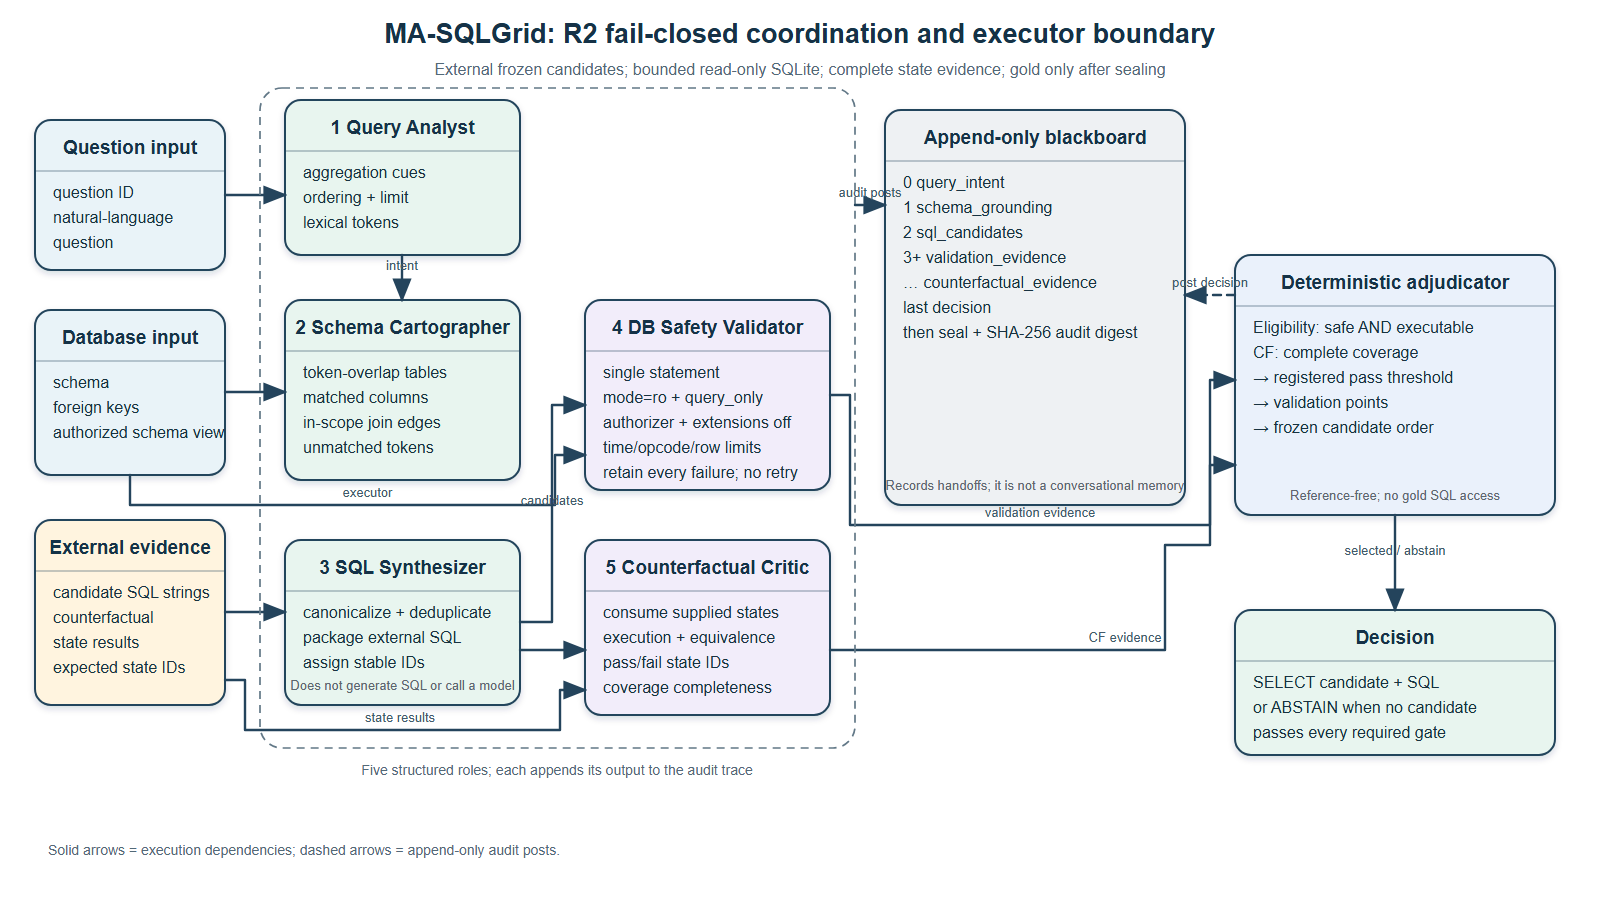
\includegraphics[width=0.98\textwidth]{figures/fig_ma_sqlgrid_implemented_coordination_r2.png}
\caption{Implemented R2 \masql{} boundary (code-native SVG and deterministic raster derivative). Candidate SQL is supplied externally. The database validator enforces read-only and resource limits; counterfactual-required selection demands complete named-state coverage; gold SQL remains outside the blackboard until sealing. User authorization and operational approval remain outside this software boundary.}
\label{fig:coordination}
\end{figure}

The \textbf{Query Analyst} produces a structured question-only intent record containing lexical tokens, detected aggregations, ordering requirements, and an explicit limit when present. It does not select SQL or see correctness. The \textbf{Schema Cartographer} maps lexical intent to tables, columns, and foreign-key edges. The current skeleton uses deterministic overlap and records unmatched tokens; a richer GridDB adapter adds disclosed domain rules and graph expansion.

The \textbf{SQL Synthesizer} packages externally produced SQL strings. It contains no model client, performs no hidden API call, canonicalizes whitespace and semicolons, removes exact duplicates without changing first occurrence, and assigns stable identifiers. The \textbf{Validation Engine} separates lexical admissibility from the executor trust boundary. The executor bound into release v3 opens a frozen database through a URI with \texttt{mode=ro\&immutable=1}, enables SQLite \texttt{query\_only}, disables loadable extensions, and installs an authorizer that admits selection, reads, selected functions, and recursive-query opcodes. Writes, DDL, transactions, attachments, pragmas, metadata enumeration, dangerous file/extension functions, and reads outside configured table/column allowlists are denied. A progress handler enforces registered time and opcode limits, and result fetching enforces a row cap. Every attempt records database and SQL hashes, authorization or resource failure, elapsed time, row count, and result hash; no automatic retry removes a failure.

R3 adds an auditable executor variant with explicit function allowlisting, maximum projected width, maximum scalar-cell bytes, and maximum total returned-result bytes. Ten additive tests pass, including oversized scalar/result and wide-projection denial. These R3 controls were implemented after release v3 and were \emph{not} used to obtain its 5760-attempt ledger or 80/100/101 counts. A SQL table/column allowlist is a query-scope mechanism supplied by the caller; it is not authentication, identity management, row-level access control, or proof that a particular utility user is entitled to the data. Both versions therefore establish tested SQLite mutation denial and bounded execution only, not user authorization, data minimization, process isolation, or operational approval.

The \textbf{Counterfactual Critic} consumes named state results, rejects duplicate state identifiers, and records evaluated, passed, failed, and missing states. When counterfactual evidence is optional, missing evidence remains diagnostic and does not break prior no-counterfactual behavior. When the caller requires counterfactual evidence, coverage must equal the complete registered state set and the pass threshold must be met; otherwise the candidate is ineligible. Thus an incomplete 1/1 record cannot outrank a complete 10/11 record. Existing formal-v5 labels compare predictions with gold and remain forbidden during selection.

\subsection{Deterministic Adjudication and Abstention}

Eligibility always requires safety and successful execution. The default rule assigns 40 validation points for safety, 40 for execution, 10 for question-derived aggregate-shape conformity, 5 for question-derived ordering conformity, and up to 5 for lexical value hits. In no-counterfactual mode, ties preserve original candidate order. In required-counterfactual mode, incomplete coverage fails closed before ranking and the registered pass threshold is enforced. If no candidate remains eligible, the controller abstains. These are deterministic recorded engineering rules, but v3 does not establish that their design preceded access to derived outcomes for the 180 items. Weight, pass-threshold, and reversed-order results are therefore descriptive sensitivity analyses.

For this paper, robustness is a vector rather than a universal label (Table~\ref{tab:robustness}). Only tested components are reported as evidence.

\begin{table}[htbp]
\caption{Operational robustness dimensions and their evidence boundaries.}
\label{tab:robustness}
\centering
\small
\resizebox{\textwidth}{!}{%
\begin{tabular}{p{2.4cm}p{4.0cm}p{3.8cm}p{3.3cm}}
\toprule
Dimension & Registered operation/end point & Evidence in this paper & Not established\\
\midrule
Mutation safety & DB-enforced denial of write/DDL/attach/pragma operations & Adversarial executor tests; unchanged database hash & User authorization or whole-process sandboxing\\
Resource boundedness & Timeout/opcode and maximum-row termination & Recursive-query and row-overflow tests; retained failure traces & Worst-case bounds for every SQLite feature\\
Evidence completeness & Complete named-state set required before CF-aware eligibility & Fail-closed tests and complete three-state ledgers & Missing-not-at-random state correction\\
Metamorphic invariance & Selected result equals T0 under irrelevant-relation, index/rebuild, and nullable-extension witnesses & 180-question offline selector result & Value drift, paraphrase, production-state, or semantic robustness\\
Semantic validity & Agreement with frozen GridDB reference after board sealing & Finite historical-pool accuracy & Qualified human gold or field-operational correctness\\
\bottomrule
\end{tabular}}
\end{table}

\begin{algorithm}[htbp]
\caption{Gold-isolated deterministic coordination}
\label{alg:coordination}
\begin{algorithmic}[1]
\REQUIRE question $x_i$, schema $S_i$, external candidates $\mathcal{Y}_i$, read-only executor, named state evidence
\STATE post structured intent and schema grounding to the append-only blackboard
\STATE canonicalize and deduplicate externally produced candidates
\FOR{each candidate $y\in\mathcal{Y}_i$}
  \STATE apply single-statement read-only validation
  \STATE record execution and available reference-free state evidence
\ENDFOR
\IF{required named-state coverage is incomplete for a candidate}
  \STATE mark that candidate ineligible (fail closed)
\ENDIF
\IF{no safe executable candidate meets all registered gates}
  \STATE abstain
\ELSE
  \STATE apply the fixed validation, state-evidence, coverage, and order rule
\ENDIF
\STATE post the decision and seal the blackboard
\STATE load reference results only for offline evaluation
\end{algorithmic}
\end{algorithm}

\subsection{Inherited GridDB Factorial Design}

The paired design crosses context package $c\in\{0,1\}$ and composite hint $h\in\{0,1\}$. F00 uses full DDL and global values without the hint; F01 adds the hint; F10 uses compact domain-grounded context without the hint; and F11 combines compact context and the hint. The same 180 questions appear in all four cells for each backbone, yielding 720 Qwen and 720 Granite predictions.

Qwen2.5-Coder-7B Q4\_K\_M and Granite-3.3-8B Q4\_K\_M were run at temperature zero with fixed snapshots. Each prompt produced exactly one response. The parser retained the first SQL candidate through the first semicolon; the validator then applied the read-only policy. There was no candidate ranking, multi-agent negotiation, or repair in this experiment.

Strict execution equality is primary. A common-target projected-column indicator is a secondary manipulation check. Paired finite-set contrasts use normalized-SQL clusters as dependence proxies, registered sign-flip tests, composition-sensitivity bootstrap intervals, and Holm correction. The intervals describe sensitivity to the observed corpus composition, not population confidence.

\subsection{Component, Multi-State, and Public Protocols}

The separately frozen component study contains 700 scored calls. E1 compares candidate generation with and without presented value evidence. E2 requests up to three candidates and compares a deterministic reference-answer-independent selector with the first candidate. Selection is sealed before gold loading. Rescue, harm, and oracle-at-three are descriptive; oracle-at-three is a gold-only upper-bound diagnostic.

The v5 reliability protocol reproduced all 1440 T0 labels and then executed every prediction over 18 states. The primary 66-question analysis uses a logical-AND endpoint over 15 semantic states. A prediction passes only when it agrees with the reference on every included state. The nine registered contrasts form a separate Holm family; with only 12 structural clusters, all $2^{12}=4096$ sign assignments are enumerated.

The BIRD protocol compares direct prompting, decomposition, schema selection, and bounded execution repair. Each method has a fixed call pattern and zero retries. Pairwise differences use exact database-cluster sign randomization across 11 databases and Holm correction.

\subsection{Retrospective Offline Coordination Diagnostic}

The replay verifies SHA-256 for two 720-row prediction ledgers and the 25,920-row formal-v5 ledger before reading them. For each question it pools the eight existing outputs from two backbones and four prompt cells, canonicalizes SQL, and removes duplicates. Frozen T0 fields provide execution and metadata-shape evidence. The Critic records counterfactual evidence as unavailable because existing state-agreement labels are gold-relative.

This is a coverage diagnostic. Candidates were generated under different models and prompt packages; the pool is not a deployable, matched multi-agent run. No selected output is compared with gold to produce an accuracy number.

\subsection{Deterministic Descriptive Offline Re-Execution Study v3}

The R2 v3 study reuses exactly eight frozen source slots for each of the 180 GridDB evaluation questions: four Qwen prompt cells followed by four Granite prompt cells. It performs no LLM call and creates no new question or SQL label. Before any method selects, the three methods share one precomputed eight-by-four execution ledger: T0 plus three metamorphic witnesses for every slot. Thus 5760 is the shared physical evidence-collection count, not a separate natural runtime cost assigned to each selector. The fixed-order control then ignores the collected ranking evidence and chooses slot 0; validation-only passes an empty counterfactual mapping and ranks validation evidence only; the full condition requires complete 3/3 reference-free metamorphic invariance. Incomplete coverage or no passing candidate causes abstention.

The three query-blind witnesses have distinct SHA-256 values and are built from T0 without reading questions, prompts, predictions, scores, or gold. M1 adds an irrelevant relation and rows; M2 adds harmless indexes and rebuilds storage; M3 adds nullable probe columns to three business tables. M1 and M2 preserve original-schema denotation. M3 preserves explicitly projected original columns but deliberately allows wildcard projection to fail. Query order is preserved when candidate SQL contains \texttt{ORDER BY}; otherwise rows are compared as a multiset. The selector sees only question text extracted from frozen prompt ledgers, the schema, eight SQL strings, executor traces, and T0-to-witness equivalence. It does not see gold SQL, answer-shape metadata, correctness, difficulty, feature tags, required literals, or gold-relative formal-v5 labels.

Before v3 execution, a content-bound UTC timestamp, configuration, question-only prompt-derived selection view, two 720-row prediction ledgers, schema, T0, three witness databases, complete witness manifest, exact witness-builder bytes and SHA-256, executor, coordinator, core and release runners, all four regression-test files, and the passing pre-run test record were bound into a 21-\emph{artifact} manifest with content SHA-256 \texttt{8b34bc370451173197ad07b460908537836409d6eb49f303caf46d13d53889e6}. The number 21 denotes manifest entries, not test cases. The restored frozen tree passes 30/30 tests across four files: 10 agent, 9 release-v3, 4 replay, and 7 executor tests. The additive R3 executor suite passes 10/10 tests, of which seven preserve earlier cases and three are new test methods; these counts must not be added as 40 independent tests. A transient 33/33 count produced while the frozen executor path had been overwritten was invalid, was reverted, and is excluded from the evidence record. The witness manifest independently binds its builder and three database hashes. Within each v3 run, all 180 blackboards and their decisions were sealed and written before that execution path directly loaded raw gold. Each run retains all 1440 source slots and all $180\times8\times4=5760$ shared attempts, including failures, without retry. Runs v3a and v3b produced byte-identical selection, evaluation, sensitivity, and summary files. Independent release audit passed mechanical integrity and descriptive traceability but failed the prior-outcome-independence evidence-class gate: the frozen pre-run test suite had opened v2 gold-derived evaluation rows for these same 180 items. The machine-readable \texttt{SUPERSESSION\_NOTICE.json} controls interpretation and invalidates conflicting prospective fields in the immutable historical configuration, summaries, and internal 29/29 mechanical audit. V3 is therefore deterministic descriptive re-execution, not a scientific release independent of prior same-item outcomes. V1 and v2 remain preserved diagnostic predecessors and are excluded from claims.

Descriptive endpoints are strict execution accuracy over all 180 questions, coverage and abstention, complete metamorphic invariance of the selected candidate, and rescue/harm relative to fixed order. The retained sensitivity matrix crosses three weight policies, invariant-pass thresholds of 1/3, 2/3, and 3/3 while always requiring complete observation, and original versus reversed candidate-order tie breaking. Because same-item outcomes were accessible before v3, this matrix is reported only as descriptive analysis.

\section{Results}

\subsection{Complete GridDB Cell Results}

All 1440 scheduled predictions are present, and independent SQLite re-execution reproduced the stored execution verdicts. Table~\ref{tab:cells} reports strict execution equality.

\begin{table}[htbp]
\caption{Strict execution equality over 180 GridDB questions per cell.}
\label{tab:cells}
\centering
\small
\setlength{\tabcolsep}{4pt}
\begin{tabular}{lcccc}
\toprule
Backbone & F00 full/no hint & F01 full/hint & F10 compact/no hint & F11 compact/hint\\
\midrule
Qwen & 76/180 (0.4222) & 129/180 (0.7167) & 78/180 (0.4333) & 108/180 (0.6000)\\
Granite & 77/180 (0.4278) & 100/180 (0.5556) & 74/180 (0.4111) & 108/180 (0.6000)\\
\bottomrule
\end{tabular}
\end{table}

\begin{figure}[htbp]
\centering

\includegraphics[width=0.94\textwidth]{figures/results/fig01_v2_cells.pdf}
\caption{Audited GridDB cell point estimates. Each cell contains all 180 attempts; the figure is descriptive and does not replace registered factorial contrasts.}
\label{fig:cells}
\end{figure}

The common-target projected-column diagnostic is 0.5222 in F00 for both backbones. Qwen obtains 0.9667, 0.5889, and 0.9611 in F01, F10, and F11; Granite obtains 0.8778, 0.5667, and 0.9222. Returning the requested number of columns is therefore easier than returning the intended rows. In Qwen F01, projected-column conformity is 0.9667 while execution equality is 0.7167.

\subsection{Factorial Effects and Multiplicity}

For Qwen, the composite-hint execution effect is +0.2306, the package--hint interaction is $-0.1278$, and the compact-package main effect is $-0.0528$. Granite's corresponding estimates are +0.1583, +0.0611, and +0.0139. Zero of nine primary execution tests survives Holm correction. Qwen's hint effect has raw/adjusted $p=0.01372/0.09604$, its interaction $0.00919/0.07352$, and the cross-backbone hint modifier $0.00640/0.05760$. No primary factorial execution effect or modifier is therefore described as statistically nonzero.

In the separately corrected secondary family, the common-target hint effects survive: +0.4083 for Qwen (adjusted $p=0.000090$) and +0.3556 for Granite (adjusted $p=0.01944$). Because the hint supplies structural information later scored by this endpoint, these are manipulation-check results, not independent semantic evidence.

\subsection{Component Results}

The component run completed all 700 scored calls. Presented value evidence increased Qwen first-candidate execution equality by +0.1059 over 170 eligible questions (95\% composition-sensitivity interval [+0.0282, +0.2013], adjusted $p=0.0310$). Granite's estimate was zero with an interval spanning zero. The cross-backbone modifier did not meet the registered rule, so the Qwen result is not replicated across backbones.

The deterministic selector changed 24 Qwen and 36 Granite choices. Relative to the first candidate, it rescued eight and harmed one Qwen question, and rescued ten while harming none for Granite. Execution effects were +0.0389 and +0.0556; neither survived its two-test Holm family. Oracle-at-three values of 0.6389 and 0.4667 are gold-only diagnostics and are not deployable selector results.

\begin{table}[htbp]
\caption{Complete component endpoints from the 700-call audited prospective component protocol. V0 contains the 170 value-intervention-eligible questions; V1 contains all 180. These are component, not five-role, outcomes.}
\label{tab:componentcounts}
\centering
\small
\resizebox{\textwidth}{!}{%
\begin{tabular}{llrrr}
\toprule
Backbone & Condition & First correct & Selector correct & Oracle@3 diagnostic\\
\midrule
Qwen & V0 no value evidence & 83/170 (0.4882) & 83/170 (0.4882) & 100/170 (0.5882)\\
Qwen & V1 with value evidence & 105/180 (0.5833) & 112/180 (0.6222) & 115/180 (0.6389)\\
Granite & V0 no value evidence & 69/170 (0.4059) & 69/170 (0.4059) & 72/170 (0.4235)\\
Granite & V1 with value evidence & 71/180 (0.3944) & 81/180 (0.4500) & 84/180 (0.4667)\\
\bottomrule
\end{tabular}}
\end{table}

\begin{figure}[htbp]
\centering

\includegraphics[width=0.92\textwidth]{figures/results/figure_01_primary_effects.pdf}
\caption{Prospectively frozen component effects. Intervals describe composition sensitivity; the registered decision also requires multiplicity-adjusted evidence.}
\label{fig:components}
\end{figure}

\subsection{Multi-State Reliability Results}

The v5 scorer produced all 25,920 registered rows, and its T0 slice reproduced 1440/1440 snapshot labels. Across the 66-question automatic subset, 15-state logical-AND rates range from 0.6212 (Granite F01) to 0.8182 (Granite F00). All nine Holm-adjusted values equal 1.0000 under exact cluster-sign enumeration. No context, hint, interaction, or cross-backbone multi-state effect meets the declared rule. These rates characterize agreement over constructed witness states, not population accuracy or human-certified equivalence.

\begin{table}[htbp]
\caption{Complete 15-state logical-AND counts for the prediction-blinded 66-question automatic subset.}
\label{tab:multistatecounts}
\centering
\small
\begin{tabular}{lcccc}
\toprule
Backbone & F00 & F01 & F10 & F11\\
\midrule
Qwen & 49/66 (0.7424) & 48/66 (0.7273) & 53/66 (0.8030) & 43/66 (0.6515)\\
Granite & 54/66 (0.8182) & 41/66 (0.6212) & 51/66 (0.7727) & 49/66 (0.7424)\\
\bottomrule
\end{tabular}
\end{table}

\begin{figure}[htbp]
\centering
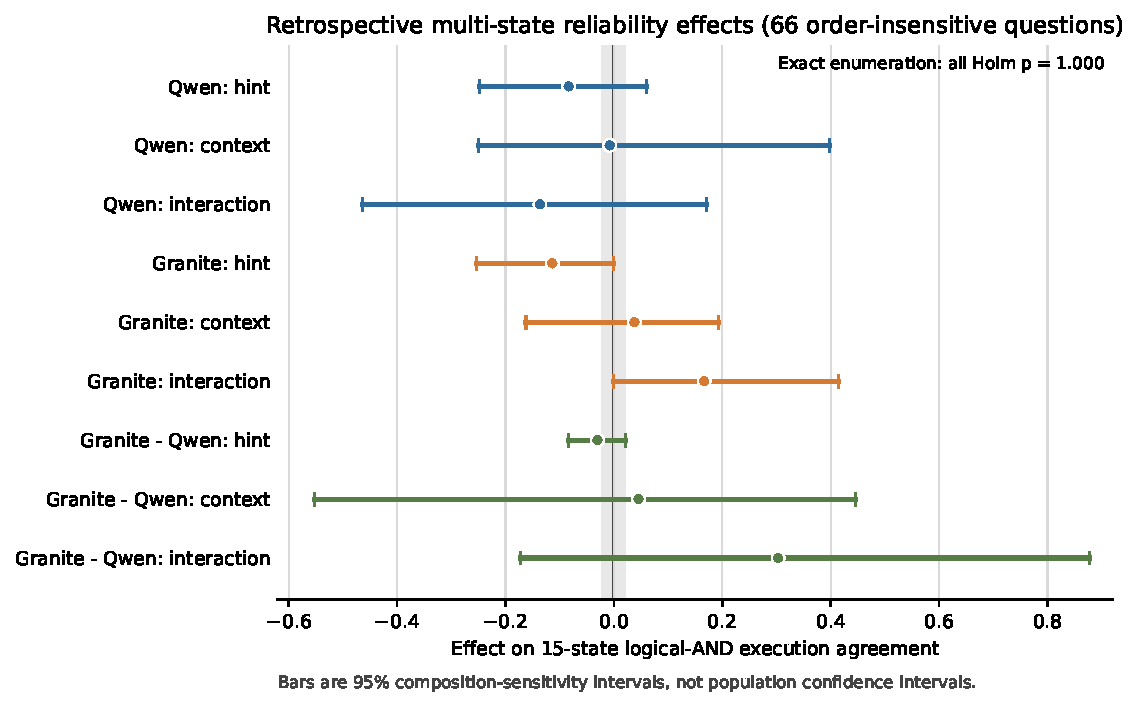
\includegraphics[width=0.92\textwidth]{figures/results/fig04_semantic_reliability.pdf}
\caption{GridDB multi-state logical-AND agreement for the prediction-blinded automatic subset. The endpoint is a constructed-state robustness diagnostic.}
\label{fig:multistate}
\end{figure}

\subsection{Public BIRD Results}

Table~\ref{tab:bird} reports all eight cells. BIRD Mini-Dev is a public non-grid portability benchmark and does not validate power-grid semantics. B0--B2 use one physical generation call per item; B3 uses two, so the inherited comparison estimates frozen workflow efficacy under unequal call counts rather than a call-matched repair effect. Each backbone completed 2500 calls, 2000 final predictions, zero retries, and zero final-ledger omissions; latency and token totals were not promoted into the retained summary and are therefore reported as unavailable rather than reconstructed.

\begin{table}[htbp]
\caption{Inherited BIRD Mini-Dev v1.1 results (non-grid portability evidence; 11 database clusters). Intervals are database-cluster composition-sensitivity intervals.}
\label{tab:bird}
\centering
\small
\setlength{\tabcolsep}{3pt}
\begin{tabular}{llrrrrp{1.5cm}}
\toprule
Backbone & Method & Correct/500 & Accuracy & Interval & Calls/item & Failures\\
\midrule
Qwen & B0 direct & 189/500 & 0.378 & [0.286, 0.470] & 1 & 0 final omissions\\
Qwen & B1 decomposition & 151/500 & 0.302 & [0.203, 0.401] & 1 & 0 final omissions\\
Qwen & B2 schema selection & 197/500 & 0.394 & [0.279, 0.511] & 1 & 0 final omissions\\
Qwen & B3 execution repair & 174/500 & 0.348 & [0.250, 0.452] & 2 & 0 final omissions\\
Granite & B0 direct & 102/500 & 0.204 & [0.125, 0.284] & 1 & 0 final omissions\\
Granite & B1 decomposition & 105/500 & 0.210 & [0.131, 0.294] & 1 & 0 final omissions\\
Granite & B2 schema selection & 101/500 & 0.202 & [0.137, 0.273] & 1 & 0 final omissions\\
Granite & B3 execution repair & 118/500 & 0.236 & [0.159, 0.318] & 2 & 0 final omissions\\
\bottomrule
\end{tabular}
\end{table}

After Holm adjustment, Qwen decomposition is 0.076 below direct prompting (adjusted $p=0.0430$), and schema selection is 0.092 above decomposition (adjusted $p=0.0117$). No Granite contrast survives correction. Different method orders across the two model snapshots argue against a universal prompting recipe. The two failed incident runs totaling 2476 physical calls remain excluded and immutable; they are not retries contributing to these denominators.

\subsection{Retrospective Replay Coverage}

The replay audited all 180 GridDB questions without a generation call. At least two distinct frozen SQL candidates were present for 173 questions. After safety checks and binding to consistent T0 execution evidence, 172 questions had at least two eligible candidates and entered retrospective adjudication. Seven failed closed because only one unique SQL remained, and one failed because fewer than two candidates were eligible.

\begin{table}[htbp]
\caption{Retrospective offline coordination diagnostic coverage. Counts are not accuracy and do not estimate multi-agent improvement.}
\label{tab:replay}
\centering
\begin{tabular}{lr}
\toprule
Coverage gate & Questions\\
\midrule
Audited & 180\\
At least two unique frozen SQL candidates & 173\\
At least two eligible candidates & 172\\
Retrospectively adjudicated & 172\\
Failed closed: one unique candidate & 7\\
Failed closed: fewer than two eligible candidates & 1\\
Reference-free counterfactual evidence available & 0\\
\bottomrule
\end{tabular}
\end{table}

Unique candidate counts ranged from one to eight: 1 (7 questions), 2 (19), 3 (15), 4 (18), 5 (27), 6 (23), 7 (45), and 8 (26). These counts show that frozen assets can populate the coordination interfaces for most questions. They do not show that retrospectively selected SQL is correct. No retrospective accuracy, execution gain, rescue rate, or multi-agent superiority is reported.

\subsection{Descriptive Offline Coordination-Selection Results}

The deterministic descriptive re-execution retained 5760 candidate--state attempts; 332 were non-executable or authorization/resource/SQL failures and remained in the all-attempt ledger. Every question nevertheless had at least one eligible candidate, so both adjudicating selectors covered 180/180 questions and abstained on 0/180. Table~\ref{tab:offline} reports the recorded rules.

\begin{table}[htbp]
\caption{New v3 offline selection over one historical eight-slot pool per question. All methods choose after the same shared precomputed 32-attempt evidence collection. Accuracy is finite-corpus strict execution equality after all blackboards were sealed; this is not a new-generation or five-role end-to-end experiment.}
\label{tab:offline}
\centering
\small
\resizebox{\textwidth}{!}{%
\begin{tabular}{lrrrrrr}
\toprule
Selector & Correct/180 & Accuracy & Covered & Abstained & Invariant & Rescue/harm\\
\midrule
Fixed order, equal budget & 80/180 & 0.4444 & 180 & 0 & 177/180 & 0/0\\
Validation rank, equal budget, no CF & 100/180 & 0.5556 & 180 & 0 & 179/180 & 22/2\\
Complete metamorphic coordination & 101/180 & 0.5611 & 180 & 0 & 180/180 & 23/2\\
\bottomrule
\end{tabular}}
\end{table}

The two adjudicating selectors each had more than one highest-scoring candidate on 130/180 questions (Table~\ref{tab:ties}). Their mean top-tie multiplicities were 5.4000 and 5.3889. All eight candidates tied on 79 validation-only questions and 78 complete-witness questions. With original-order tie breaking, 178/180 selections came from Qwen source slots; this reflects source order, not a learned preference or semantic advantage.

\begin{table}[htbp]
\caption{Complete top-score tie diagnostic for the two adjudicating selectors. Multiplicity distributions are reported as ``tie size:number of questions''.}
\label{tab:ties}
\centering
\small
\resizebox{\textwidth}{!}{%
\begin{tabular}{lrrlp{5.2cm}}
\toprule
Selector & Tied questions & Mean size & Multiplicity distribution & Selected source-slot counts\\
\midrule
Validation only & 130/180 & 5.4000 & 1:50; 2:5; 3:3; 4:4; 5:5; 6:8; 7:26; 8:79 & Qwen F00/F01/F10/F11: 115/49/12/2; Granite F00/F10: 1/1\\
Complete witnesses & 130/180 & 5.3889 & 1:50; 2:5; 3:3; 4:4; 5:5; 6:9; 7:26; 8:78 & Qwen F00/F01/F10/F11: 114/50/12/2; Granite F00/F10: 1/1\\
\bottomrule
\end{tabular}}
\end{table}

Validation-only ranking added 20 net correct items relative to fixed order through 22 rescues and 2 harms. Complete-witness selection changed the chosen candidate on only Q039, yielding one further frozen-reference match (101/180 versus 100/180), one additional rescue, no additional harm, and no coverage or abstention change. Table~\ref{tab:q039} gives the complete constructed trace.

\begin{table}[htbp]
\caption{Q039 is the sole validation-only versus complete-witness selection difference. Correctness is agreement with the frozen synthetic reference, not an independently adjudicated engineering judgment.}
\label{tab:q039}
\centering
\footnotesize
\resizebox{\textwidth}{!}{%
\begin{tabular}{p{2.5cm}p{4.6cm}p{4.6cm}p{2.2cm}}
\toprule
Field & Validation-only & Complete witnesses & Interpretation\\
\midrule
Natural-language request & \multicolumn{2}{p{9.2cm}}{``Show the first scheduled work order after June 2024.''} & Ambiguous: ``after June'' can imply after 30 June, and ``scheduled'' can denote a status or merely a scheduled date.\\
Selected query & \texttt{SELECT * FROM work\_orders WHERE scheduled\_date > '2024-06-01' ORDER BY scheduled\_date ASC LIMIT 1} & \texttt{SELECT work\_order\_id, scheduled\_date FROM work\_orders WHERE scheduled\_date > '2024-06-01' ORDER BY scheduled\_date ASC LIMIT 1} & Both omit an explicit scheduled-status predicate and use a date boundary whose intended meaning lacks expert adjudication.\\
M3 outcome & Fails when nullable columns extend wildcard width & Preserves the explicit two-column projection & Constructed projection-stability behavior\\
Frozen-reference match & Incorrect & Correct & Outcome-exposed 1/180 trace only\\
\bottomrule
\end{tabular}}
\end{table}

M3 added nullable columns to \texttt{work\_orders}; consequently, complete-witness eligibility rejected the wildcard projection and retained the explicit \texttt{work\_order\_id, scheduled\_date} projection. Because neither query resolves the request's status and date-boundary ambiguity through qualified review, this observation is not called an engineering correctness rescue. It is a synthetic, outcome-exposed projection-stability trace, not evidence of general counterfactual reasoning, semantic validity, robustness, coordination, or five-role benefit.

Table~\ref{tab:sensitivity} reports all 18 sensitivity cells. Every original-order cell produced 101/180; reverse order produced 117/180 under default and intent-emphasis weights and 118/180 under validation-equal weights. These more favorable values are outcome-exposed diagnostics, not preferred alternatives. The 16--17-item shift and high tie multiplicity show that the apparent selector behavior is materially order-dependent.

\begin{table}[htbp]
\caption{All 18 complete-witness selector sensitivity cells. Each row contains the original- and reverse-order cells for one weight/threshold combination; coverage is 180/180 throughout.}
\label{tab:sensitivity}
\centering
\small
\resizebox{\textwidth}{!}{%
\begin{tabular}{lrrr}
\toprule
Weight policy & Minimum witness passes & Original order correct/180 & Reverse order correct/180\\
\midrule
Default & 1/3 & 101 (0.5611) & 117 (0.6500)\\
Default & 2/3 & 101 (0.5611) & 117 (0.6500)\\
Default & 3/3 & 101 (0.5611) & 117 (0.6500)\\
Intent emphasis & 1/3 & 101 (0.5611) & 117 (0.6500)\\
Intent emphasis & 2/3 & 101 (0.5611) & 117 (0.6500)\\
Intent emphasis & 3/3 & 101 (0.5611) & 117 (0.6500)\\
Validation equal & 1/3 & 101 (0.5611) & 118 (0.6556)\\
Validation equal & 2/3 & 101 (0.5611) & 118 (0.6556)\\
Validation equal & 3/3 & 101 (0.5611) & 118 (0.6556)\\
\bottomrule
\end{tabular}}
\end{table}

The full machine-generated numerical supplement binds all eight GridDB cells, 12 component endpoints, eight 15-state cells, 18 sensitivity cells, the 360-row item-level tie ledger, selected-origin counts, Q039 trace, source paths, hashes, and byte counts in \texttt{R3\_EVIDENCE\_TABLES.json} and companion CSV files. This result supports auditability and exposes a design risk; it does not establish a generally robust or superior selector.

\section{Discussion}

\subsection{What the Evidence Supports}

The combined evidence supports four bounded findings. First, explicit structural and SQL-operation instructions strongly alter projected-column adherence, but surface conformity does not establish correct execution. Second, the audited prospective 700-call component experiment finds that presented value evidence matters for one frozen Qwen snapshot while showing no effect for Granite; this is component evidence, not a five-role outcome. Third, candidate selection and prompting are backbone-dependent: the component selector did not meet its registered efficacy rule, and the descriptively best BIRD method differed between Qwen and Granite. Fourth, on the historical eight-slot pool, validation ranking changed the observed finite-set score relative to fixed order, but complete witness evidence changed only Q039, and top-score ties on 130/180 items made results strongly dependent on arbitrary source order.

These findings justify separating intent, schema grounding, synthesis, validation, and state evidence. They do not establish that five roles are superior to one call or that newly generated multi-agent candidates would reproduce the offline gain. The architecture's demonstrated value is methodological and safety-bounded: typed contracts, database-enforced eligibility, complete-evidence gates, deterministic selection, abstention, incident retention, and a sealed gold boundary make later comparisons reproducible and falsifiable.

\subsection{Interpreting the Retrospective Replay}

The replay asks whether inherited ledgers contain enough distinct executable candidates to exercise the coordination interfaces. For 172 of 180 questions, they do. This reduces implementation risk and identifies eight fail-closed cases that require a registered fallback or a new matched generation policy.

The replay cannot estimate a coordination effect. Its pool mixes two backbones and four prompt packages, so generation condition and diversity are confounded. It also lacks reference-free counterfactual equivalence evidence. Post hoc gold scoring of selected outputs would remain exploratory and cannot substitute for a prospective matched comparison.

\subsection{Interpreting the Descriptive Re-Execution}

The release-v3 study hash-binds the selection view, rules, code, tests, and state inputs and verifies the software fact that each execution path directly loaded raw gold only after all blackboards were sealed. This does not establish outcome blindness: its frozen test suite had accessed gold-derived v2 evaluation rows for the same items before v3. The additive supersession notice is the first authority for interpreting the immutable release package and invalidates its historical prospective, prespecified, and outcome-unseen labels. The study is therefore a deterministic descriptive re-execution over a historical candidate pool. Equal candidate budget means that each selector received the same eight pre-existing slots; it does not mean equal historical model calls between source conditions, and it does not turn those candidates into contemporaneous agent outputs.

The small contrast between validation-only and complete-witness selection is a mechanism trace, not a gain estimate. V3 uses three different query-blind database hashes and exercises an irrelevant-relation witness, an index/storage witness, and a nullable schema-extension witness. These are constructed operator families rather than independent samples from a deployment population. The full gate changes only Q039 because M3 exposes wildcard-projection arity while preserving explicit-column projections. The natural-language request itself admits unresolved status and date-boundary interpretations, so the frozen-reference match cannot be promoted to power-grid semantic correctness. An earlier v1 diagnostic used three same-hash insertion files and is retained as an excluded incident; v2 is retained as a provenance-incomplete predecessor. The supersession notice excludes their prospective interpretations and none of these predecessors supports the current scientific claim.

The tie audit quantifies a second limitation: 130/180 questions have multiple highest-scoring candidates for each adjudicating selector, with approximately 5.4 candidates in the average top-tie set. The original-order rule consequently chooses source slots without semantic evidence and selects Qwen-origin candidates on 178/180 items. Reporting only the 0.5556 default or choosing the 0.6556 reverse-order sensitivity after outcome access would be misleading. A later rule-development study requires development-only calibration, richer reference-free evidence, and a genuinely untouched evaluation resource.

\subsection{Power-Grid Use and Reproducibility}

Database-enforced read-only execution, resource limits, syntactic validity, and result-shape conformity are necessary safeguards, not operational certification. A safely executed query can still return the wrong assets, omit time bounds, misinterpret codes, or mishandle ties. Table/column/function allowlists constrain SQL operations inside this local evaluator; user authorization requires a separately authenticated identity, institutional access policy, and data-owner decision. The additive R3 cell-byte, result-byte, and output-width controls were not used in release v3 and cannot be invoked to reinterpret its results. Multi-state witnesses reduce accidental snapshot equality but cannot cover all distributions or schema changes. Generated SQL and returned source rows require authorized human inspection before any maintenance, protection, dispatch, or asset-management decision.

Negative results are part of the contribution. Zero of nine primary factorial execution tests survives correction. The deterministic component selector meets its efficacy rule for neither snapshot. No registered multi-state effect survives correction. Granite and Qwen do not share the same best BIRD method. Immutable ledgers, direct re-execution, registered test families, portable manifests, and explicit incidents preserve these outcomes rather than collapsing them into a success narrative.

\section{Limitations and Future Work}

The primary domain corpus is one synthetic database with eight tables, 98 rows, and 180 evaluation questions. Its evaluation partition was visible during development. The 70 structural groups are dependence proxies, and 58 are singletons. Results cannot be generalized to production schemas, permissions, missing-data patterns, units, access-control policies, or workloads.

Only two quantized local snapshots were evaluated. Model family, size, quantization, serving software, and serialization may interact. The compact package bundles schema reduction, values, normalization, and serialization; the hint bundles projection, aggregation, grouping, ordering, and limit rules. The inherited factorial experiment identifies package effects rather than contributions of individual internal rules.

The five-role core and frozen release-v3 executor pass 30 unit/adversarial/regression tests; the separate R3 executor passes 10 additive tests, seven inherited and three new. The 21-entry freeze manifest is not a test count, and the invalid transient 33/33 run is excluded. The system has not completed a new-generation experiment on an evaluation resource whose outcomes were previously inaccessible to the study process. Its Analyst and Cartographer are deterministic skeletons, its Synthesizer packages external candidates, and its adjudication weights have not been independently optimized. Release v3 descriptively re-executes selection over historical candidates and previously evaluated items; it does not estimate generation, communication, latency, token, or autonomous-agent effects. Existing formal-v5 agreement labels are gold-relative and intentionally excluded from selection.

RTS-GMLC, SimBench, and NERC question--SQL assets remain machine-adjudicated silver data. Qualified review is required for intended projections, units, ordering, tie handling, and result granularity before external accuracy is reported.

Future work should execute a new hash-locked, call-matched comparison of four contemporaneous generation conditions: a single direct candidate; staged question/schema handoffs with one candidate; a fixed multi-candidate budget with validation and adjudication but no counterfactual evidence; and the same candidate pool with a pre-registered multi-family reference-free state suite. Model snapshot, question order, database state, decoding, candidate count, physical calls, and evaluator must be held constant. The protocol must pre-register execution accuracy, valid SQL, abstention, tokens, latency, failure taxonomy, clustered inference, multiplicity, and incident retention. The candidate-order rule must be chosen on development-only evidence before the untouched evaluation set is opened.

Further work can replace lexical grounding with a trained schema linker, add a low-confidence full-schema fallback, compare deterministic adjudication with budget-matched voting, and evaluate risk--coverage calibration. Qualified power-system/database reviewers must independently assess domain semantics; LLM or author-assisted triage cannot be relabeled as independent expert gold. Every change should receive a new protocol identity rather than modifying a completed run.

\section{Conclusions}

\masql{} reframes power-grid text-to-SQL as an auditable coordination problem. Five typed software roles separate question analysis, schema mapping, candidate packaging, safety and execution validation, and named-state criticism. A deterministic controller records their handoffs, selects only eligible candidates, and abstains when required evidence is incomplete. Here, \emph{multi-agent} denotes this inspectable role decomposition, not demonstrated benefit from five autonomous language-model agents. The frozen executor enforces read-only and resource limits at the SQLite boundary rather than relying on lexical filtering alone; R3 adds separately tested result-byte, cell-byte, width, and function controls that are not retroactive to v3.

The inherited experiments provide a substantial but bounded evidence base. The 1440-prediction GridDB study shows strong projected-column instruction uptake but no primary execution effect surviving Holm correction. The 700-call component study supports presented values for one Qwen snapshot, not Granite, and does not validate its selector under the registered rule. The 25,920-row state study finds no corrected factorial agreement effect. The 5000-call BIRD protocol supplies a non-grid public comparison whose best method depends on the backbone and whose methods use unequal call counts. The retrospective replay confirms candidate coverage for 172 of 180 questions without accuracy claims.

The descriptive offline re-execution records 80/180 for fixed order, 100/180 for validation-only, and 101/180 for complete witnesses. Both adjudicating selectors have highest-score ties on 130/180 questions, average tie multiplicity is approximately 5.4, and reverse order changes the complete-witness sensitivity result to 117--118/180. The sole Q039 difference is a constructed, outcome-exposed, semantically ambiguous projection trace. These facts, the historical mixed-source pool, development-visible GridDB, and absent qualified semantic review prevent a general multi-agent superiority or power-grid deployment claim. The original title is retained as the framework identity; \emph{robust} refers only to explicitly tested mutation-denial, bounded-execution, complete-evidence, and three-witness mechanisms, not universal or operational robustness.

\supplementary{The R3 source tree contains the machine-generated complete numerical tables, 360-row tie ledger, Q039 trace, supersession notice, executor extension and tests, response matrix, and source hashes. A final editor/reviewer archive must be generated from an explicit allowlist after R3 review and verified by clean extraction. It must exclude old-title manuscripts, old PDFs, \texttt{ROUND1\_SECTION\_DRAFT}, credentials, caches, and excluded incident outputs presented as evidence. The public repository at \url{https://github.com/gaoxingkele/ma-sqlgrid} must be synchronized and tagged before submission. Restricted materials remain governed by the Data Availability Statement.}
\authorcontributions{Conceptualization, B.L. and Y.Y.; methodology, B.L.; software, B.L.; validation, B.L. and C.S.; formal analysis, B.L. and C.S.; investigation, B.L. and C.S.; resources, Y.Y.; data curation, B.L. and C.S.; writing---original draft preparation, B.L.; writing---review and editing, C.S. and Y.Y.; visualization, B.L.; supervision, Y.Y.; project administration, Y.Y.; funding acquisition, Y.Y. All authors have read and agreed to the published version of the manuscript.}
\funding{This work is associated with grant number 521300250006. The exact funding-agency wording requires written author confirmation before submission.}
\institutionalreview{Not applicable. This study did not involve human participants or animals.}
\informedconsent{Not applicable.}
\dataavailability{The public repository at \url{https://github.com/gaoxingkele/ma-sqlgrid} must be synchronized and tagged before submission; this statement does not assert that its current contents match R3. BIRD Mini-Dev remains available from its public provider. Owing to third-party licensing restrictions, restricted source records and source-dependent RTS-GMLC or SimBench artifacts may be requested from the corresponding author for editorial and peer-review verification, subject to third-party permission and applicable licenses; reviewer access is not a redistribution license. A round-bound editor/reviewer archive must be built from the final R3 allowlist and clean-extraction verified before submission. Its inventory will distinguish public, restricted, derived, machine-silver, historical, and excluded-incident materials and bind the supersession notice, numerical supplement, code, tests, and independent audits.}
\acknowledgments{During preparation of this manuscript, the authors used OpenAI Codex (GPT-5-based) for drafting, editing, code review, and reproducibility checks. The scientific architecture and result graphics in R2 are code-native; no generative-image output is used as quantitative evidence. The authors reviewed and edited the outputs and take full responsibility for the publication. Machine-generated external question--SQL candidates were not treated as human or domain-expert ground truth.}
\conflictsofinterest{The authors declare no conflicts of interest. Confirmation of the exact funding-agency identity and funder-role statement remains a manual pre-submission action.}

\begin{adjustwidth}{-\extralength}{0cm}
\reftitle{References}
\bibliography{references_verified}
\PublishersNote{}
\end{adjustwidth}
\end{document}
